\documentclass[11pt,a4paper]{article}
\usepackage[T1]{fontenc}\usepackage[utf8]{inputenc}\usepackage[scaled=0.95]{helvet}\renewcommand{\familydefault}{\sfdefault}
\usepackage[a4paper,margin=2.2cm]{geometry}\usepackage{graphicx,booktabs,longtable,hyperref}\usepackage[hidelinks]{hyperref}
\setlength{\parindent}{0pt}\setlength{\parskip}{0.6em}
\begin{document}
{\LARGE\textbf{How wide is rue de Terrebonne? The roadway along the lane, from the City\textquoteright{}s 2015 LiDAR}}\\[4pt]
{\small Terrebonne-open-sources, 2026-11-04. Data: Ville de Montréal, LiDAR aérien 2015 and unités d\textquoteright{}évaluation foncière (open data, CC-BY 4.0). Method and code: \url{https://openmobilitydata.github.io/Terrebonne-open-sources/2015-lidar-terrebonne-street-width/}.}

\section*{Question}
The winter layout proposed for rue de Terrebonne (borough file 1266880005, adopted November 2, 2026) keeps the contraflow protected lane and turns the lane running with traffic into parking for the winter, so that cyclists going with traffic share the traffic lane. The cross-section drawn for that type of layout in the borough\textquoteright{}s 2023 study (EXP, Figure 6-6, p.~72) is, from the south property line: sidewalk 1.8 m, contraflow lane 2.0 m, buffer 0.5 m, parking 2.4 m, shared lane 3.5 m, parking 2.4 m, sidewalk 1.8 m, that is 10.8 m from curb to curb in a 14.4 m section. Whether the street is in fact 10.8 m wide, everywhere along the 2.4 km, decides how much room any winter layout has. This note measures it.

\section*{Data and method}
The City\textquoteright{}s 2015 airborne LiDAR (six 1 km tiles, NAD83(CSRS)/MTM 8; classes ground, high vegetation, building) was rasterized once for the earlier parking work: the mean elevation of ground-class returns on a 0.25 m grid along the corridor. On that surface a cross-section is sampled every 2 m along the lane\textquoteright{}s axis (the City géobase, from the lane\textquoteright{}s west end to Girouard; 1207 stations), from 16 m south to 16 m north of the axis, every 0.1 m. On each side, scanning outward from the axis, the curb is the first place between 3 and 8 m from the axis where the ground rises by at least 7 cm over 0.5 m; its position is the point of steepest rise in that window. A Montréal curb face is 10 to 15 cm high; a driveway ramp at about 1:12 rises 4 cm over 0.5 m and does not pass, though a steeper apron sometimes does. The LiDAR was flown on two weeknights with cars parked at the curbs, and under a car or a dense tree there are no ground returns; a station is kept only when both curbs are found and the width lies between 9 and 13 m (759 stations). The right-of-way is measured on the same line as the distance between the first parcel outline on each side (the City\textquoteright{}s assessment units); the sidewalk zone is the parcel line to the curb.

\section*{Results}
\begin{itemize}
\item Curb to curb: median 11.0 m over the 759 stations kept; 10\,\% of stations read under 10.7 m and 10\,\% over 12.4 m (the high tail is aprons taken for curbs). The block medians run from 10.8 to 11.35 m: the roadway is the same width along the whole lane, within a few decimetres.
\item Right-of-way: 20.09 m at every block but the Belmore stub and three lots (the 66-foot standard, 20.12 m); sidewalk zones about 4.4 m on the north side and 4.73 m on the south side (parcel line to curb, including the grass strip).
\item EXP\textquoteright{}s own statement of the existing section (report p.~50, PDF p.~61): « L\textquoteright{}emprise fonctionnelle actuelle de la rue de Terrebonne est d\textquoteright{}environ 14,6 m, soit une chaussée d\textquoteright{}environ 11 m et deux trottoirs d\textquoteright{}environ 1,8 m. » The LiDAR\textquoteright{}s 11.0 m is EXP\textquoteright{}s « environ 11 m »; EXP\textquoteright{}s 14.6 m is roadway plus paved sidewalks, not the 20.1 m right-of-way, the difference being the grass strips.
\item Against the 2023 drawing: 10.8 m of lanes and parking in an 11.0 m roadway. The winter layout fits with about 0.2 m to spare across the street. A shared lane wider than 3.5 m would have to come from the parking bands (2.4 m), the buffer (0.5 m) or the contraflow lane (2.0 m).
\item Before 2024 the street was two-way with parking on both sides; two 3.3 m lanes (EXP 2023) and two parking bands of 2.2 m make the same 11.0 m.
\end{itemize}

\begin{center}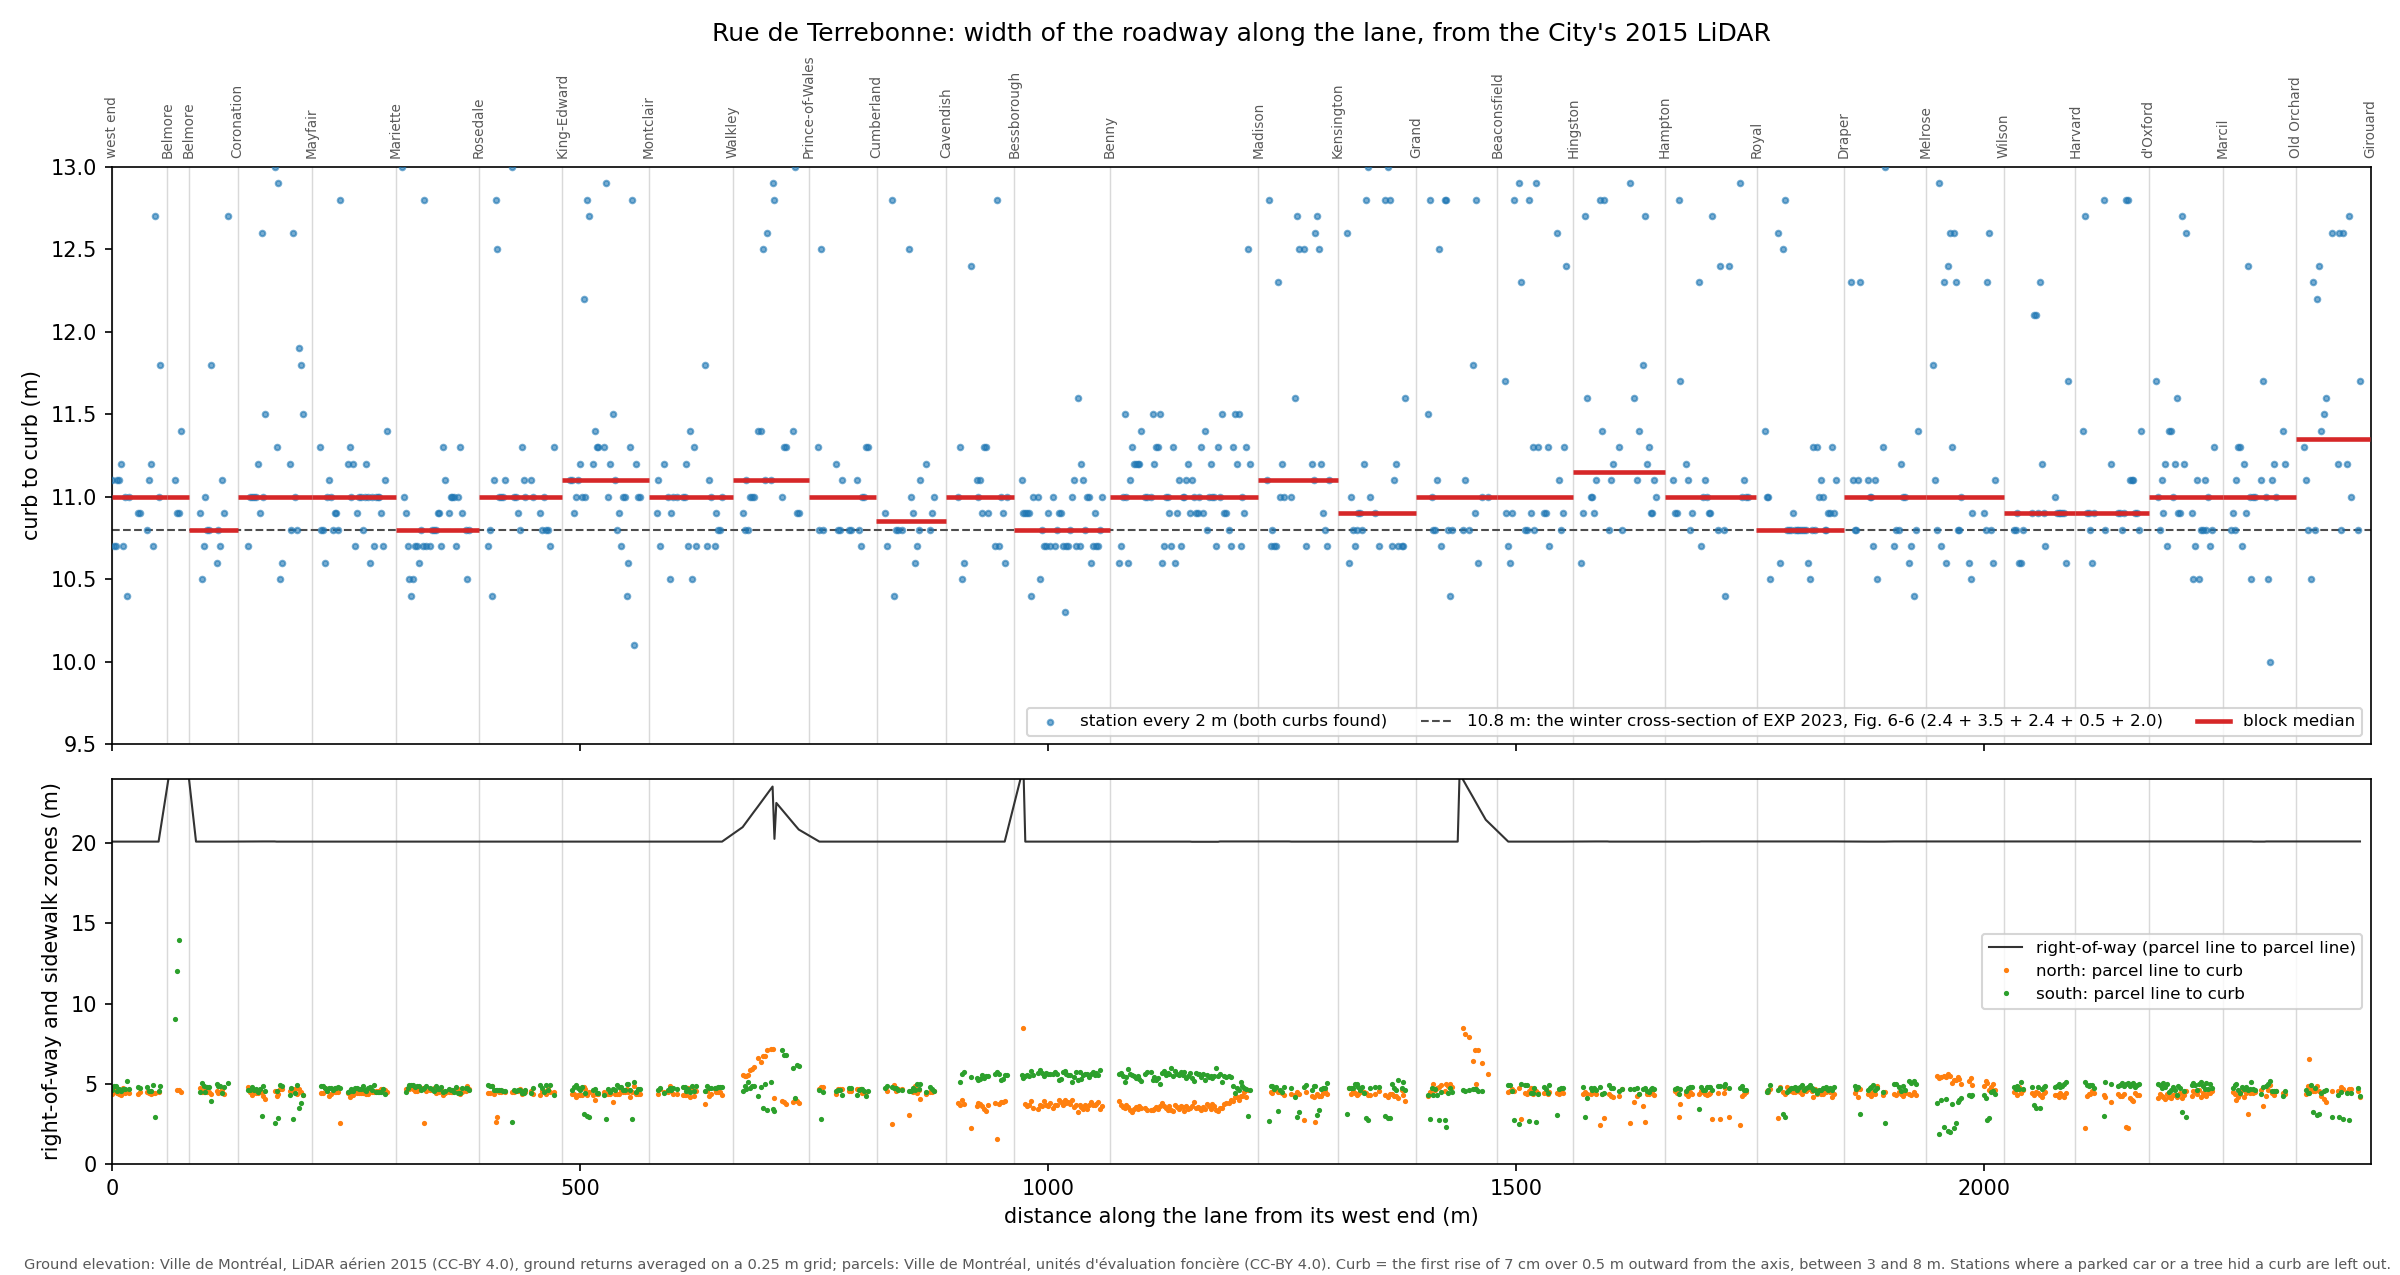
\includegraphics[width=\textwidth]{figures/street_width_profile_en.png}\end{center}
\begin{center}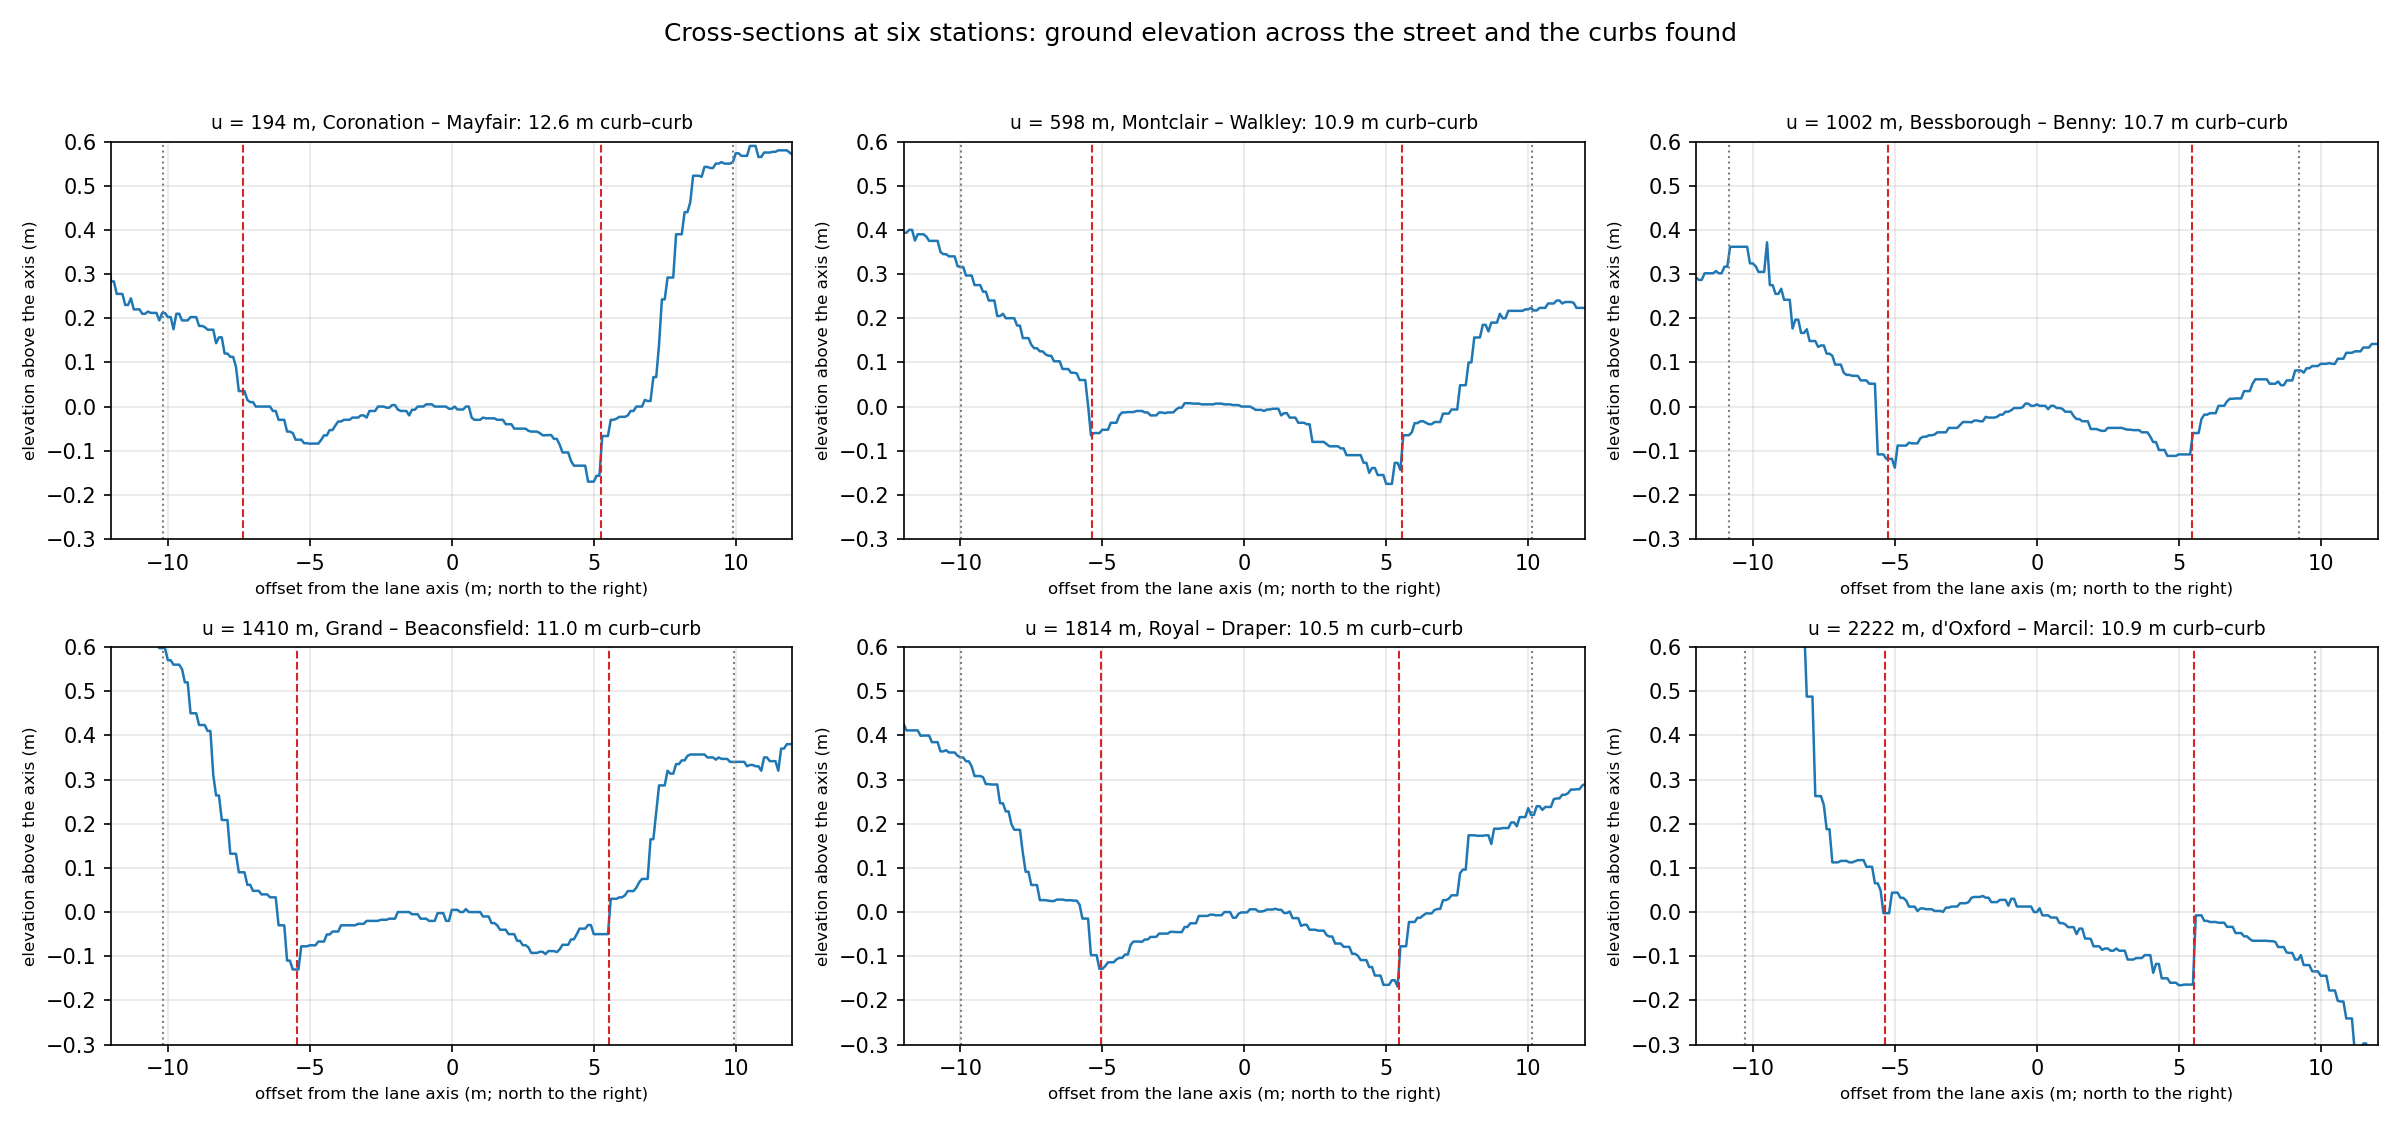
\includegraphics[width=\textwidth]{figures/street_width_sections_en.png}\end{center}
\begin{center}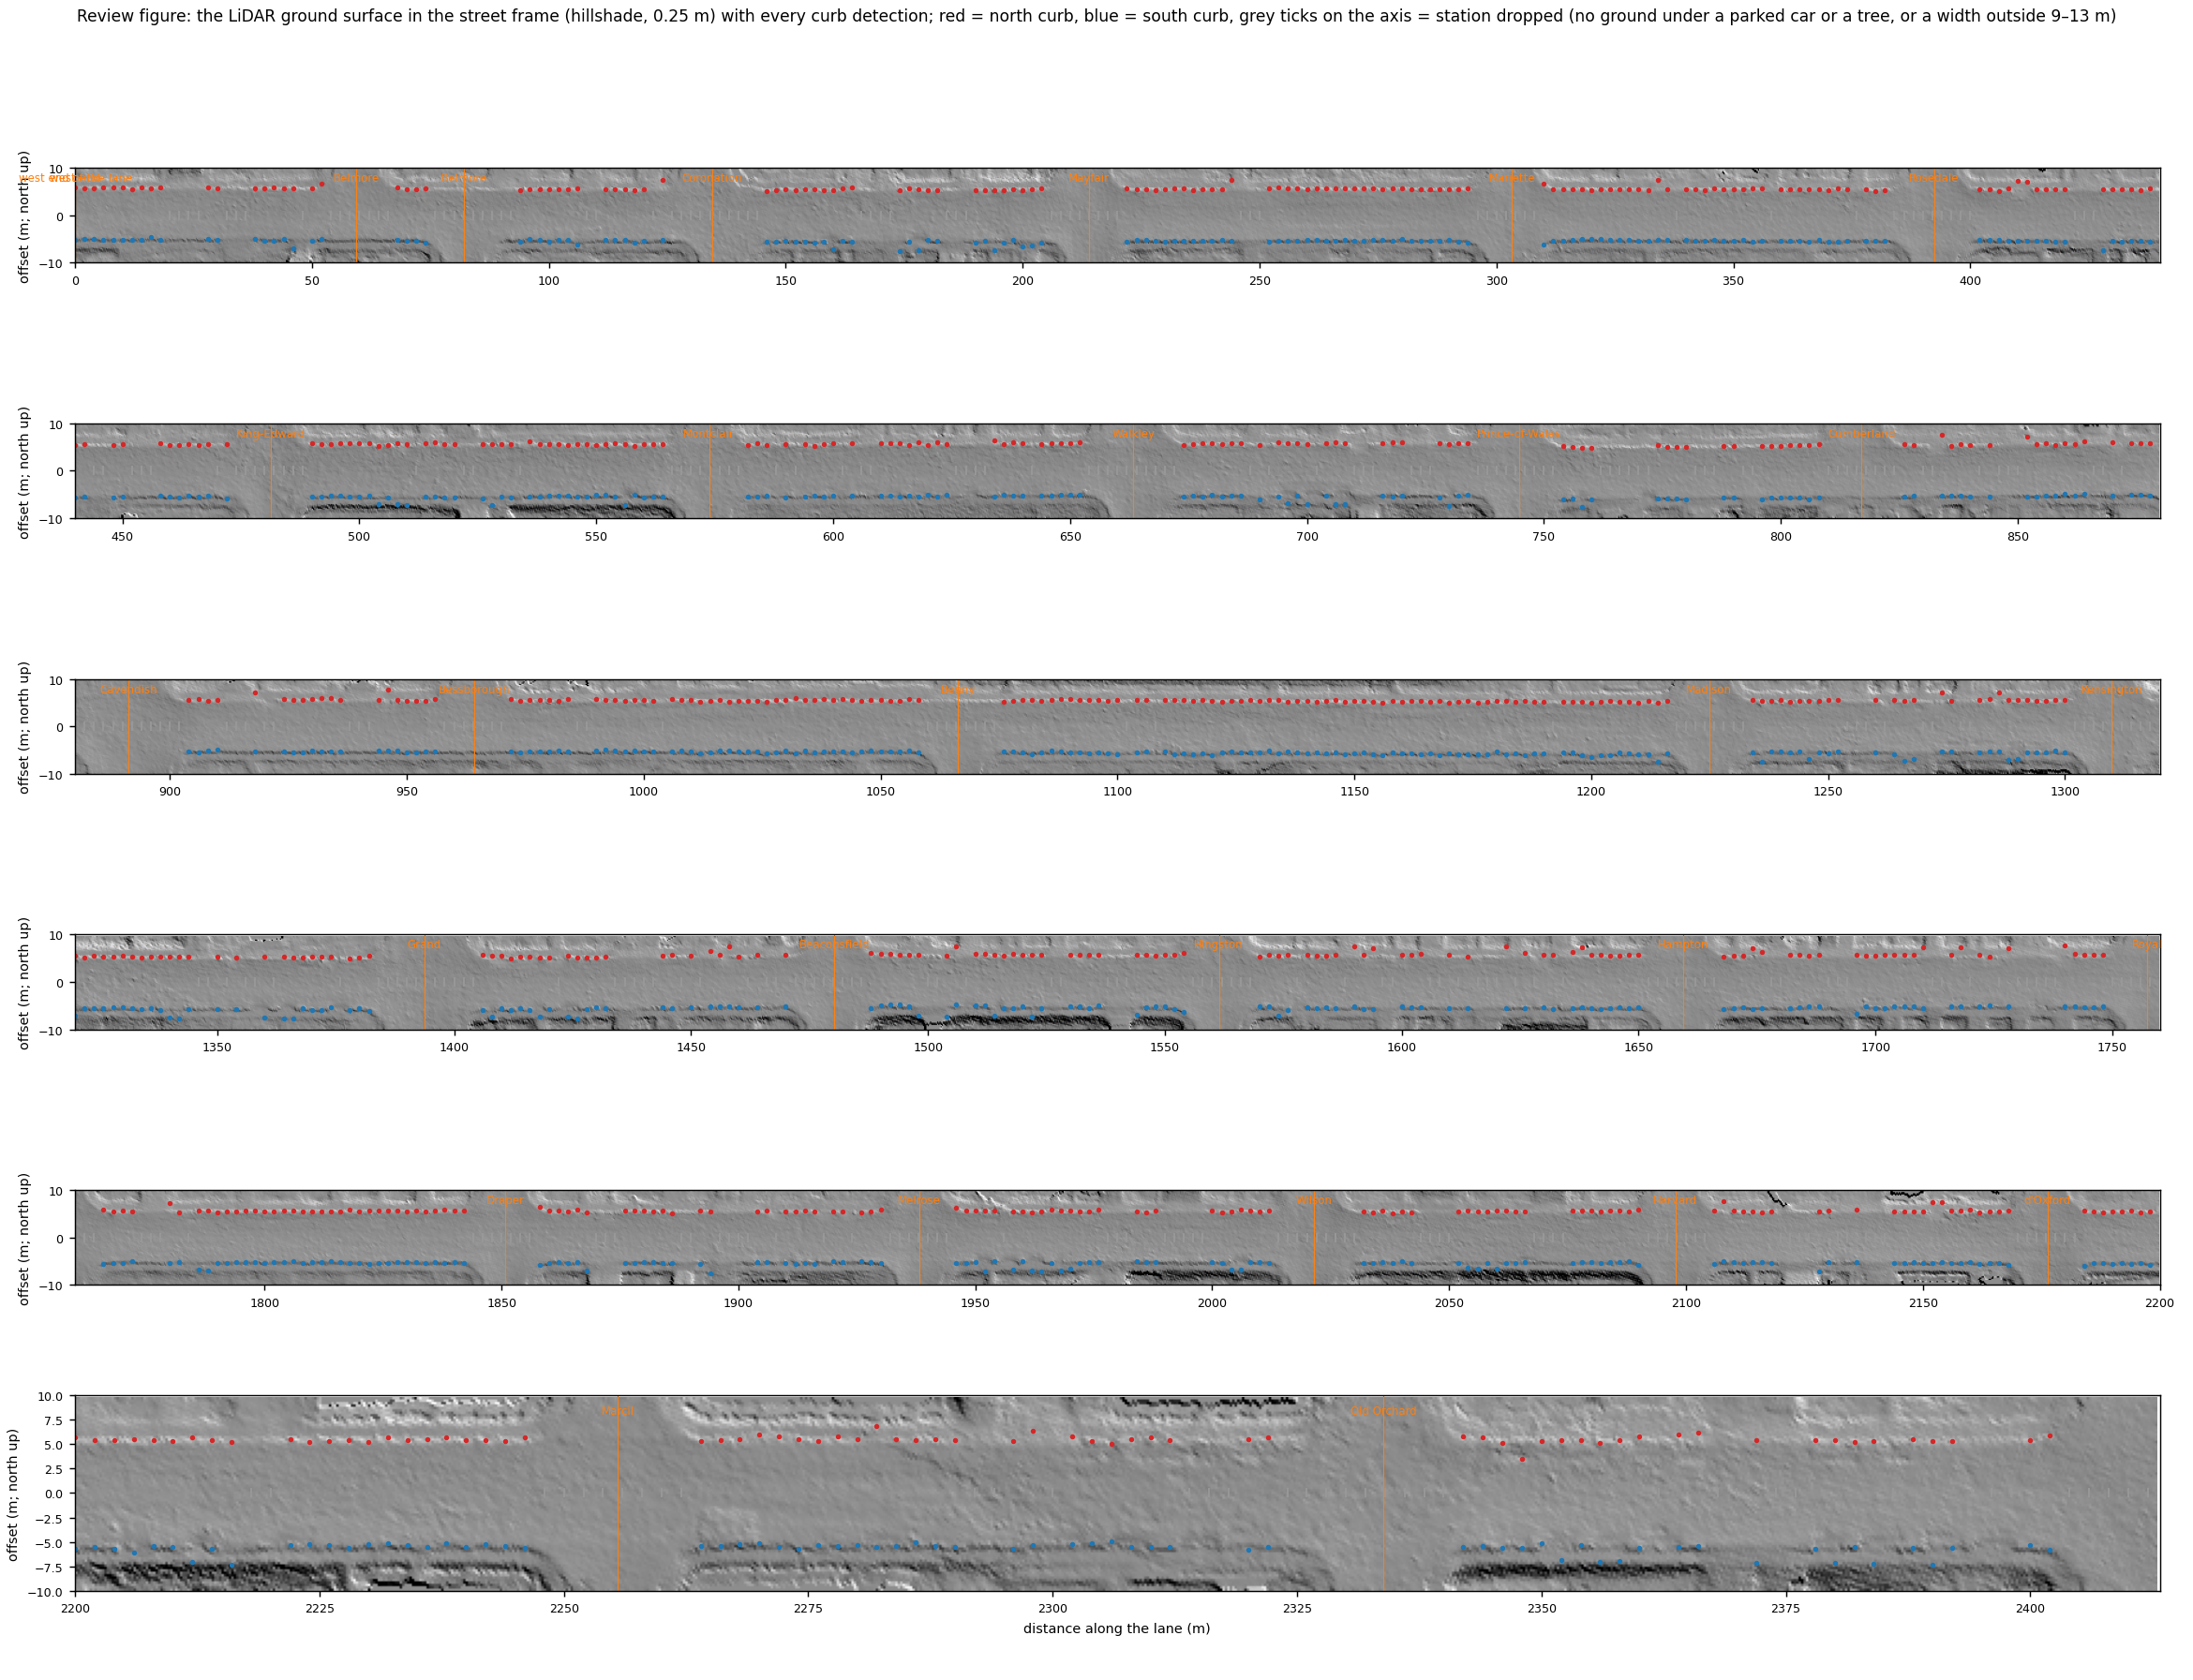
\includegraphics[width=\textwidth]{figures/street_width_overhead_en.png}\end{center}
\begin{center}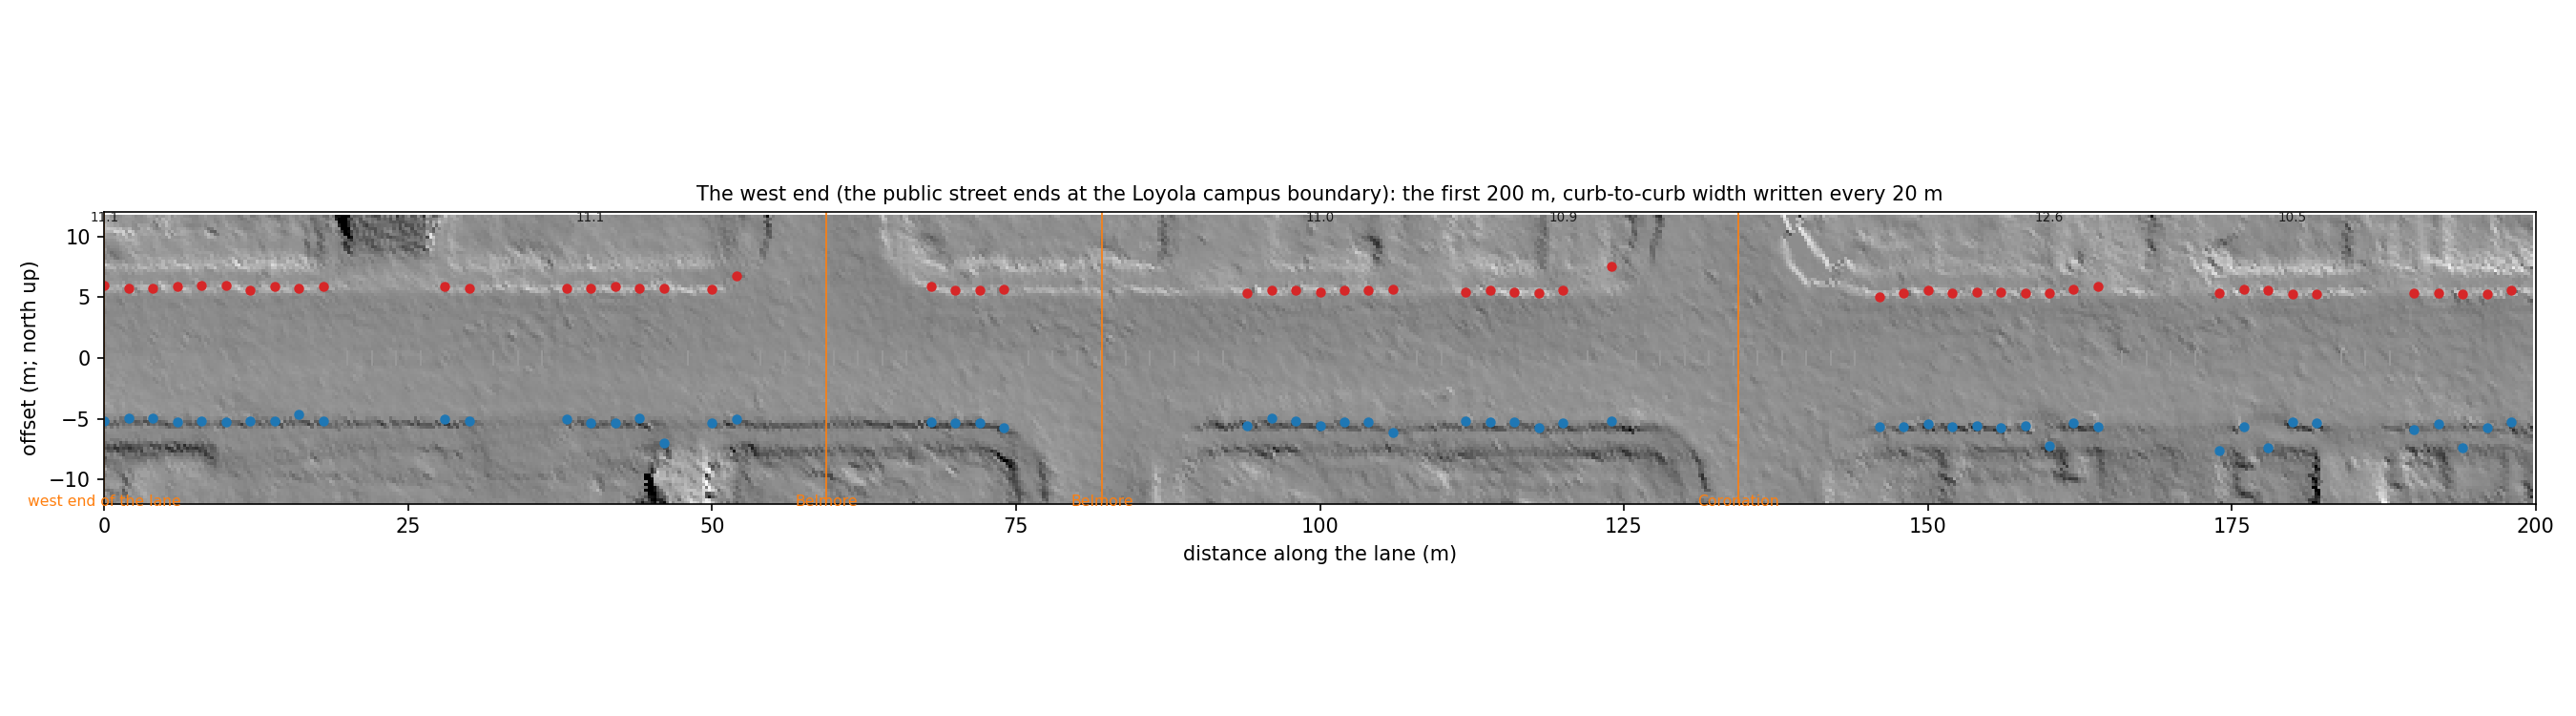
\includegraphics[width=\textwidth]{figures/street_width_west_end_en.png}\end{center}

\section*{The west end}
The public street ends where the lane ends, at the Loyola campus boundary (the City géobase\textquoteright{}s last segment, 1320365, ends there; beyond it the roadway is the campus\textquoteright{}s). The last public block, west end to Belmore, reads 11.0 m curb to curb (19 of 30 stations kept), a 20.09 m right-of-way and sidewalk zones of 4.4 m north and 4.7 m south: the same section as the rest of the street. It is two-way with no parking on either side; the 2015 surface and the pre-2024 imagery cannot measure the 2024 bike lanes, but an 11.0 m roadway holds, for example, two 2.0 m lanes with 0.5 m buffers and two 3.0 m travel lanes (arithmetic, not the marking plan).

\section*{EXP\textquoteright{}s three sections against the measured roadway}
\begin{center}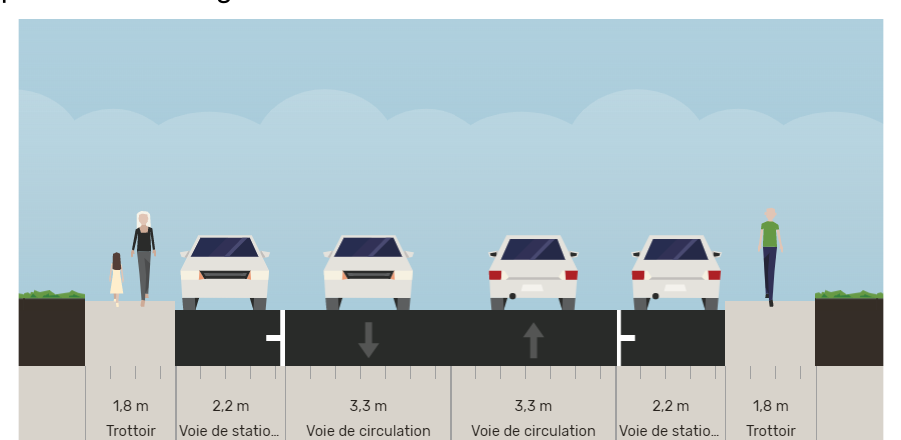
\includegraphics[width=0.75\textwidth]{../raw/exp2023_fig3-1_configuration_2023.png}\\ {\small 2023 (EXP Fig.~3-1, report p.~25): 2.2 + 3.3 + 3.3 + 2.2 = 11.0 m curb to curb.}\end{center}
\begin{center}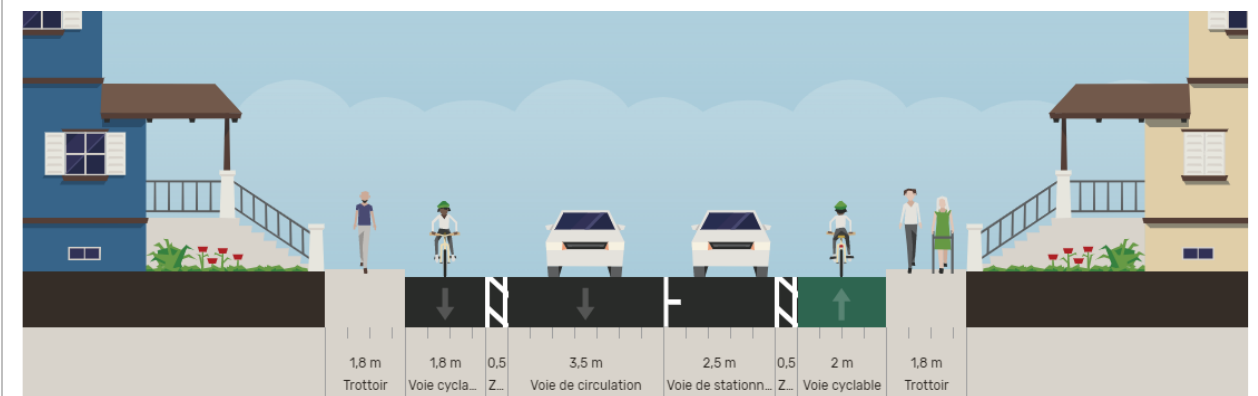
\includegraphics[width=0.75\textwidth]{../raw/exp2023_fig6-7_amenagement_B.png}\\ {\small Today, Aménagement B (Fig.~6-7, p.~72): 1.8 + 0.5 + 3.5 + 2.5 + 0.5 + 2.0 = 10.8 m.}\end{center}
\begin{center}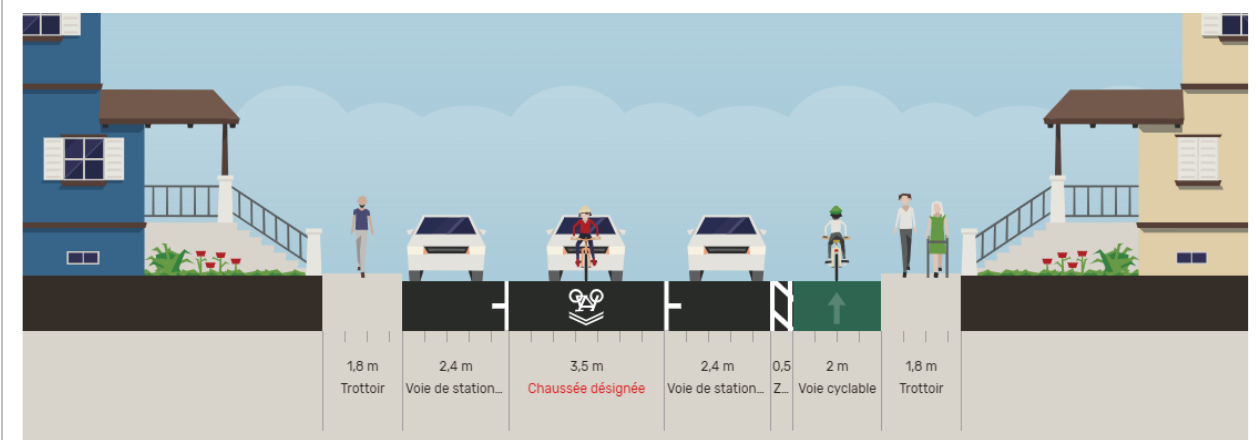
\includegraphics[width=0.75\textwidth]{../raw/exp2023_fig6-6_amenagement_A.png}\\ {\small Winter, assumed to be Aménagement A (Fig.~6-6, p.~72): 2.4 + 3.5 + 2.4 + 0.5 + 2.0 = 10.8 m; applied to B\textquoteright{}s bands, 2.3 + 3.5 + 2.5 + 0.5 + 2.0 = 10.8 m.}\end{center}
Every section EXP drew fits the measured 11.0 m with 0 to 0.2 m to spare; none has room for a wider shared lane without narrowing the parking bands, the buffer or the contraflow lane. The figures are reproduced from the borough\textquoteright{}s published study (Terrebonne-open-sources, 2023-exp-mobility-study).

\section*{The cross streets}
\textbf{Question.} Most of the streets that cross rue de Terrebonne between the lane\textquoteright{}s west end and Girouard are one-way local streets with parking on both sides and a single lane shared by cars and bicycles: the arrangement the winter layout gives the direction riding with traffic, without the contraflow lane (2.0 m) and its buffer (0.5 m). The winter section leaves 8.3 m for parking, shared lane and parking (2.4 + 3.5 + 2.4). How wide are the cross streets, and do they share a typical width?

\textbf{Method.} The same ground raster and the same curb detector, applied to the first block of each cross street on each side of Terrebonne (the géobase segments that meet the intersection), from 20 m past the intersection (clear of the curb returns) to 240 m or the block\textquoteright{}s end: a cross-section every 2 m, 14 m each side; the curb window runs 2.5 to 8 m from the axis (11 m for the three two-way boulevards, Cavendish, Grand and Girouard); a station is kept when both curbs are found and the width lies between 5 and 13 m (22 m for the boulevards). 53 blocks at 28 streets, 5,397 stations, 3,749 kept. A lowered curb at a driveway apron, or a curb hidden under a tree, makes the detector read the next rise further out, so a block\textquoteright{}s readings have a tight core and a tail toward wider values, never narrower: the figure reported per block is the most frequent reading (0.2 m bins), with the median and the 10th--90th percentiles beside it. The City\textquoteright{}s parking-sign inventory gives, for each side of each block, the number of sign poles within 12 m of the axis and the number carrying « \textbackslash{}A EN TOUT TEMPS » (no parking at any time).

\textbf{Results.}
\begin{itemize}
\item The local cross streets (47 blocks, all one-way; 46 with ten or more stations kept) read 9.0 to 9.4 m curb to curb: over all their stations the most frequent reading is 9.1 m and the median 9.4 m; block by block, 42 of 46 lie between 8.9 and 9.6 m. The others: Belmore south 8.8 m; Coronation south 7.9 m; Prince-of-Wales south 11.0 m (a 69 m stub, 10 stations); Madison north 12.5 m (42 of 110 stations kept, 33\,\% of them within 0.5 m of that reading: low confidence).
\item Every local block has parking signs on both sides but 1, with at most 3 « \textbackslash{}A EN TOUT TEMPS » poles per side (the corner clearances): parking on both sides, under the time restrictions the signs give, is the rule.
\item The three two-way boulevards are wider: Cavendish 16.5--16.6 m, Grand 15.8--15.9 m, Girouard 13.9 m.
\item Rue de Terrebonne itself: 11.0 m (most frequent reading 10.95 m, median 11.0 m), 1.6 to 2.0 m wider than its local cross streets.
\item The arithmetic. The winter section spends 2.5 m on the contraflow lane and its buffer and leaves 8.3 m for parking, shared lane and parking. A cross street of 9.0 to 9.4 m with the same two 2.4 m parking bands leaves 4.2 to 4.6 m for its shared lane. The 3.5 m shared lane the winter layout draws on Terrebonne is 0.7 to 1.1 m narrower than the lane the cross streets give the same arrangement: the cross streets are not the equivalent of the winter layout; in the part that a cyclist riding with traffic uses, they are about a metre wider.
\end{itemize}

\begin{center}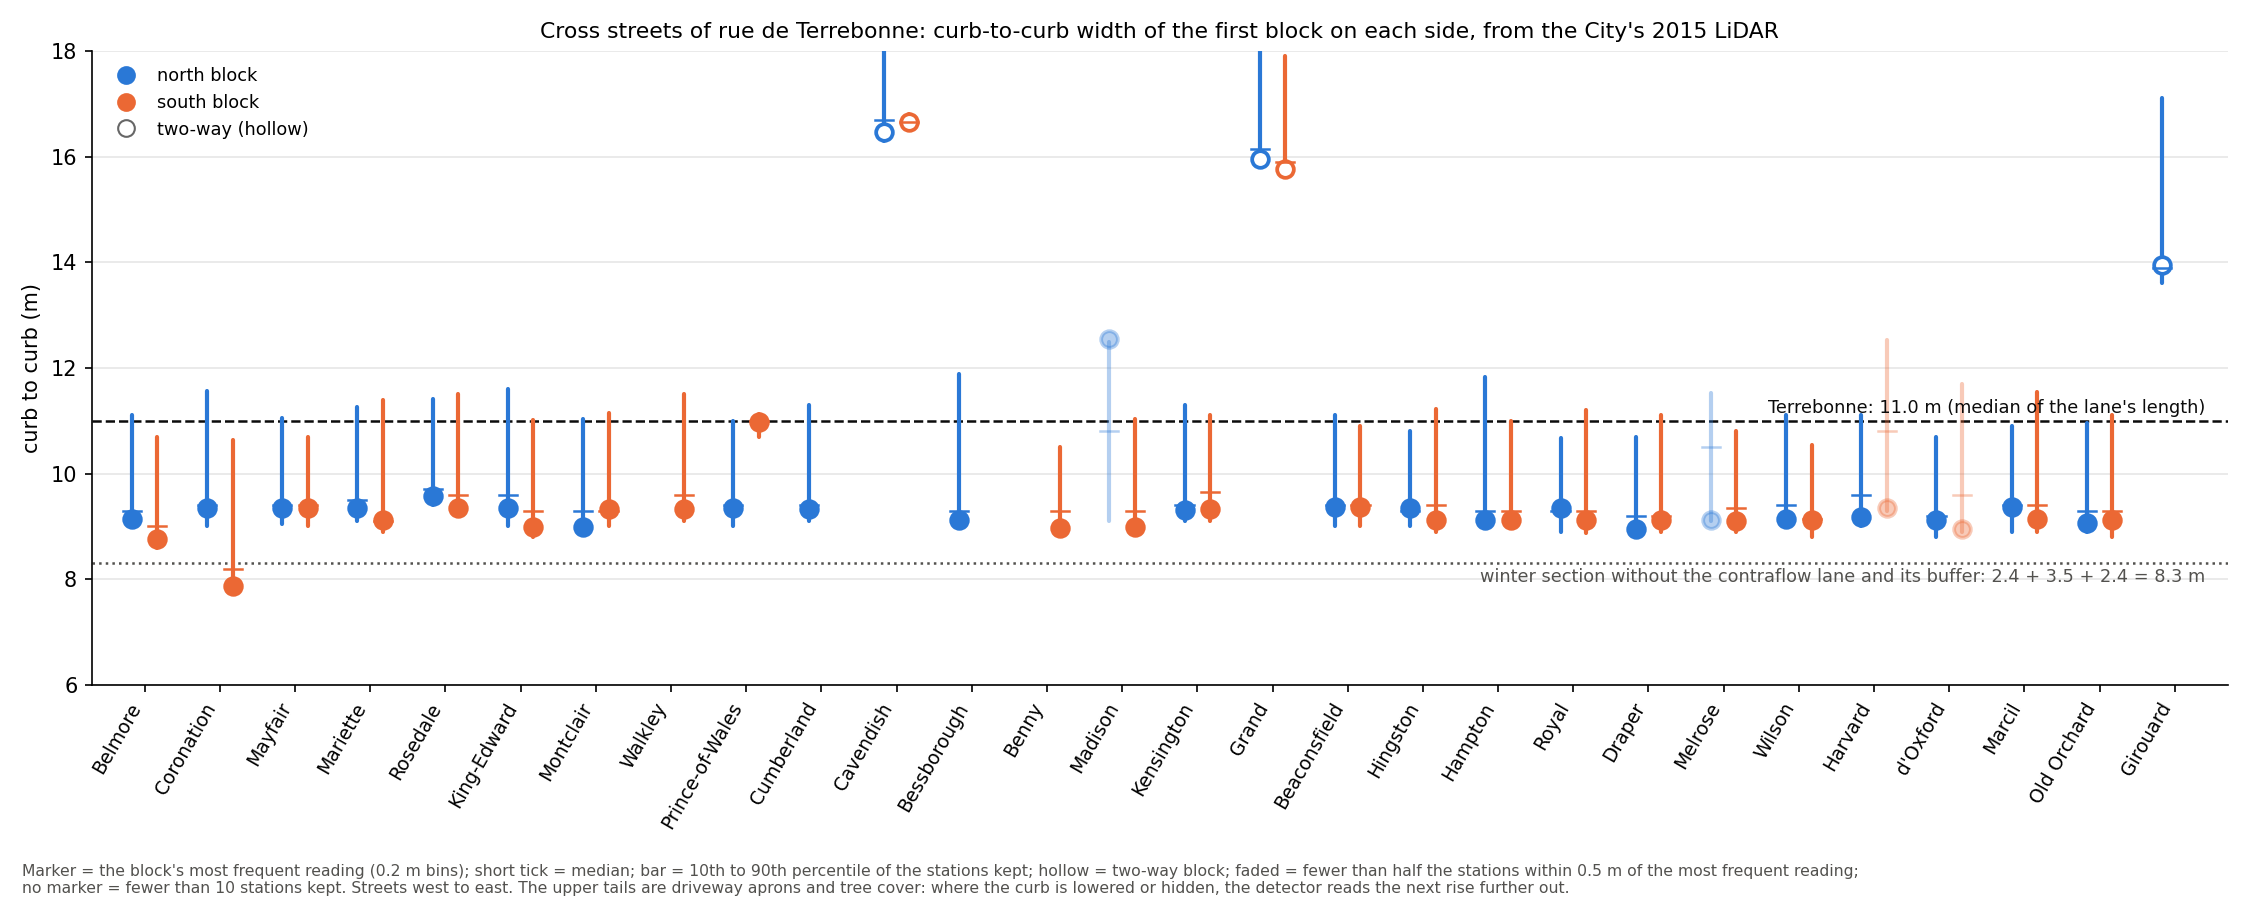
\includegraphics[width=\textwidth]{figures/cross_street_widths_en.png}\end{center}
\begin{center}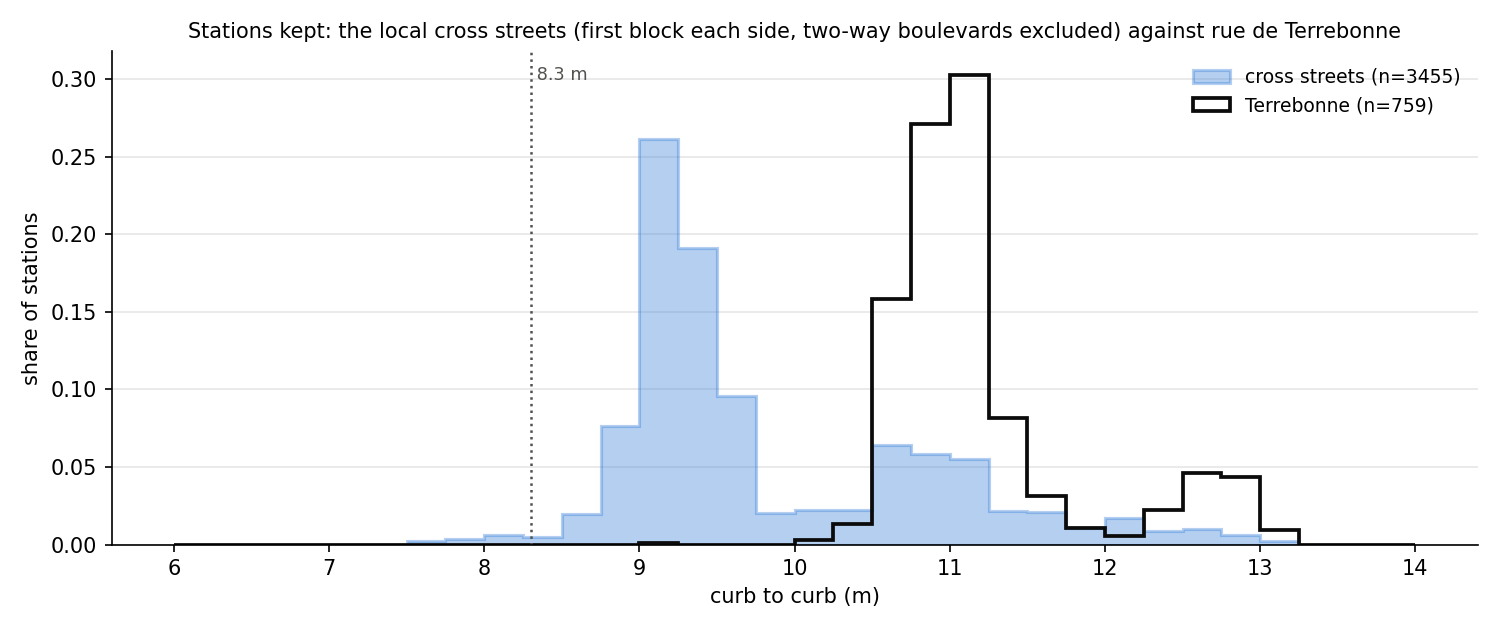
\includegraphics[width=0.85\textwidth]{figures/cross_street_widths_hist_en.png}\end{center}
\begin{center}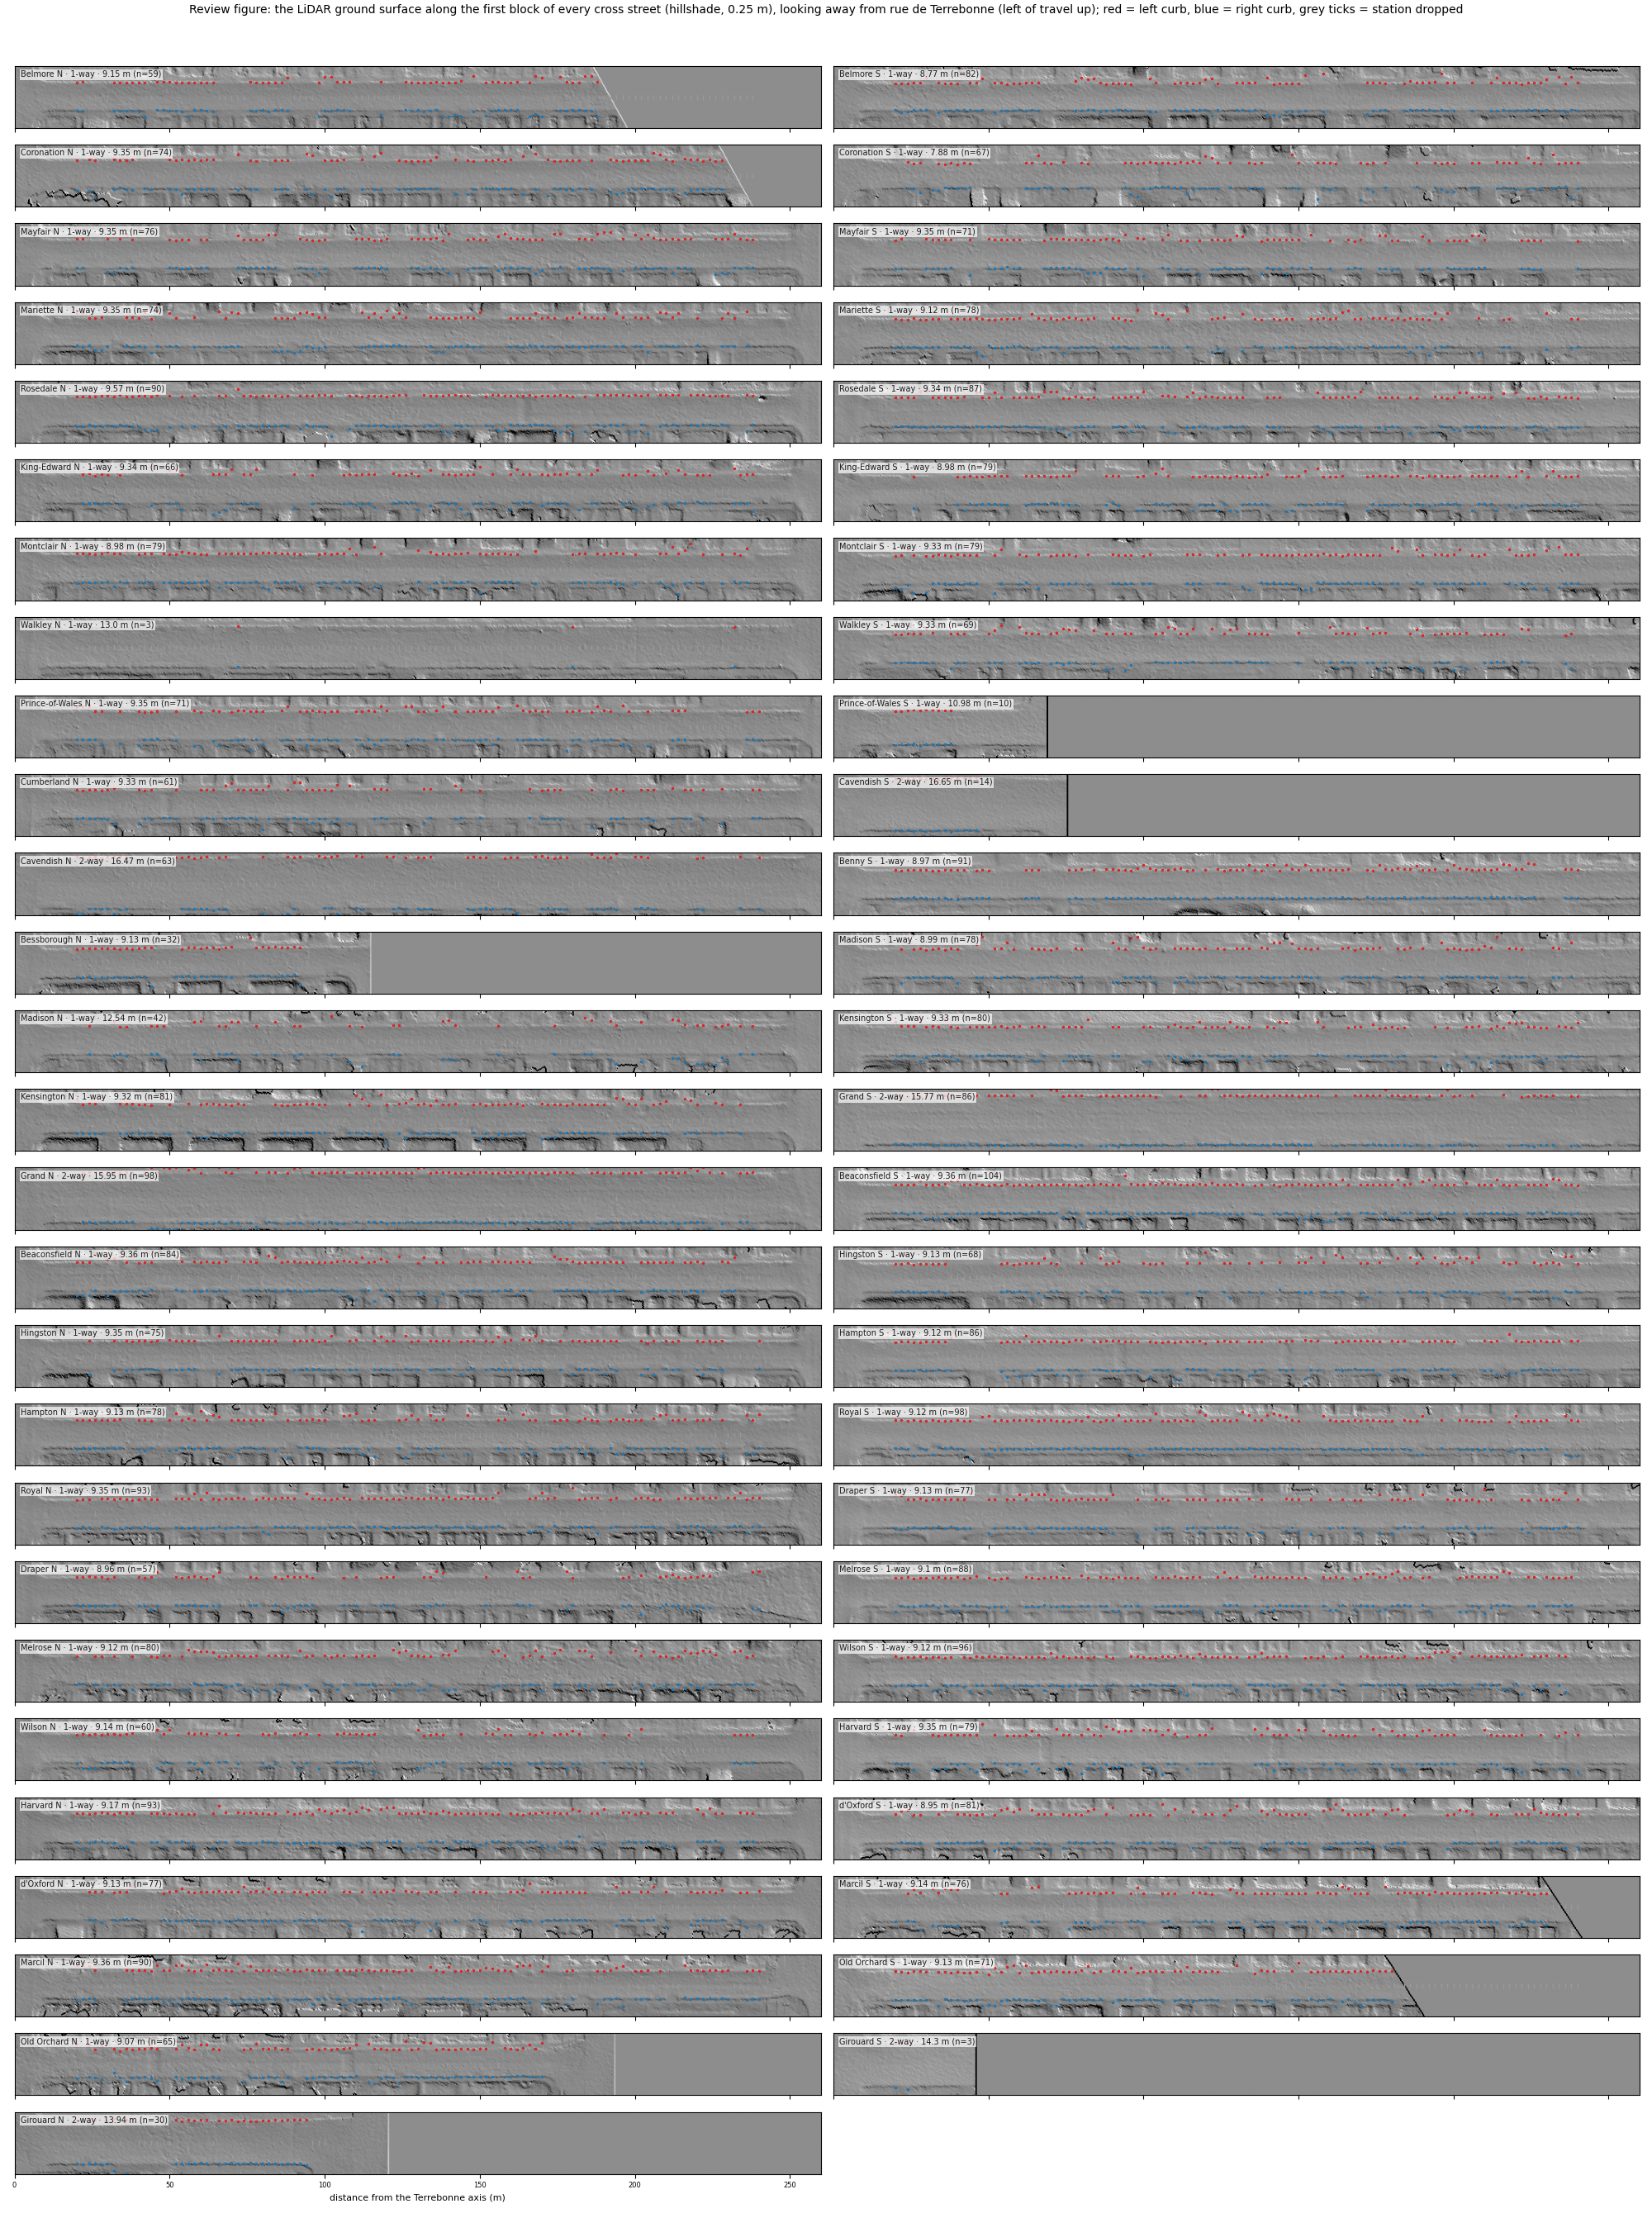
\includegraphics[width=\textwidth]{figures/cross_street_widths_review_en.png}\end{center}

\textbf{By street.} Most frequent reading / median, in metres, and the number of stations kept, for the first block north and south of Terrebonne; * = fewer than half the stations within 0.5 m of the most frequent reading; signs = parking-sign poles left + right of the block\textquoteright{}s axis, with the number of « \textbackslash{}A EN TOUT TEMPS » poles in brackets.
{\small\begin{longtable}{@{}llllll@{}}\toprule Street (west to east) & direction & north block & signs & south block & signs\\ \midrule
Belmore & one-way & 9.2 / 9.3 (59) & 5+4 (0) & 8.8 / 9.0 (82) & 5+5 (0) \\
Coronation & one-way & 9.3 / 9.4 (74) & 4+4 (1) & 7.9 / 8.2 (67) & 4+4 (1) \\
Mayfair & one-way & 9.3 / 9.4 (76) & 6+3 (0) & 9.3 / 9.4 (71) & 3+3 (0) \\
Mariette & one-way & 9.3 / 9.5 (74) & 4+7 (0) & 9.1 / 9.1 (78) & 5+4 (2) \\
Rosedale & one-way & 9.6 / 9.7 (90) & 6+2 (0) & 9.3 / 9.6 (87) & 4+3 (0) \\
King-Edward & one-way & 9.3 / 9.6 (66) & 3+6 (0) & 9.0 / 9.3 (79) & 5+6 (1) \\
Montclair & one-way & 9.0 / 9.3 (79) & 3+3 (0) & 9.3 / 9.3 (79) & 4+2 (0) \\
Walkley & one-way & -- (3) & 3+2 (4) & 9.3 / 9.6 (69) & 0+0 (0) \\
Prince-of-Wales & one-way & 9.3 / 9.4 (71) & 5+4 (0) & 11.0 / 11.0 (10) & 1+2 (0) \\
Cumberland & one-way & 9.3 / 9.4 (61) & 4+3 (0) & -- & -- \\
Cavendish & two-way & 16.5 / 16.7 (63) & 4+3 (0) & 16.6 / 16.6 (14) & 1+1 (0) \\
Bessborough & one-way & 9.1 / 9.3 (32) & 4+5 (5) & -- & -- \\
Benny & one-way & -- & -- & 9.0 / 9.3 (91) & 12+7 (2) \\
Madison & one-way & 12.5 / 10.8 (42)* & 3+3 (0) & 9.0 / 9.3 (78) & 4+3 (0) \\
Kensington & one-way & 9.3 / 9.4 (81) & 4+4 (0) & 9.3 / 9.7 (80) & 3+4 (0) \\
Grand & two-way & 15.9 / 16.1 (98) & 2+4 (0) & 15.8 / 15.9 (86) & 5+4 (0) \\
Beaconsfield & one-way & 9.4 / 9.4 (84) & 5+5 (2) & 9.4 / 9.4 (104) & 7+7 (0) \\
Hingston & one-way & 9.3 / 9.3 (75) & 5+5 (2) & 9.1 / 9.4 (68) & 4+5 (0) \\
Hampton & one-way & 9.1 / 9.3 (78) & 4+3 (1) & 9.1 / 9.3 (86) & 7+6 (0) \\
Royal & one-way & 9.3 / 9.3 (93) & 4+3 (0) & 9.1 / 9.3 (98) & 6+6 (0) \\
Draper & one-way & 9.0 / 9.2 (57) & 3+4 (1) & 9.1 / 9.2 (77) & 3+5 (1) \\
Melrose & one-way & 9.1 / 10.5 (80)* & 3+5 (0) & 9.1 / 9.3 (88) & 5+3 (0) \\
Wilson & one-way & 9.1 / 9.4 (60) & 3+4 (0) & 9.1 / 9.2 (96) & 4+4 (0) \\
Harvard & one-way & 9.2 / 9.6 (93) & 4+4 (1) & 9.3 / 10.8 (79)* & 4+4 (0) \\
d\textquoteright{}Oxford & one-way & 9.1 / 9.2 (77) & 4+3 (0) & 8.9 / 9.6 (81)* & 5+3 (1) \\
Marcil & one-way & 9.4 / 9.4 (90) & 3+6 (0) & 9.1 / 9.4 (76) & 10+6 (0) \\
Old Orchard & one-way & 9.1 / 9.3 (65) & 5+7 (2) & 9.1 / 9.3 (71) & 9+8 (2) \\
Girouard & two-way & 13.9 / 13.9 (30) & 4+2 (2) & -- (3) & 0+0 (0) \\
\bottomrule\end{longtable}}

\textbf{The comparison in one picture.} Figure~\ref{fig:boxes} draws the three widths to scale on the aerial imagery of Terrebonne and Kensington: Terrebonne from curb to curb (the block medians, 11.1 and 10.9 m), the 8.5 m that remain beside the contraflow lane and its buffer (2.5 m), where the December layout puts parking, the shared lane and parking, and Kensington from curb to curb (9.3 m, both blocks). The two Terrebonne boxes are repeated on Kensington: the 11 m box overshoots its curbs, the 8.5 m box leaves room to spare.
\begin{figure}[h]\centering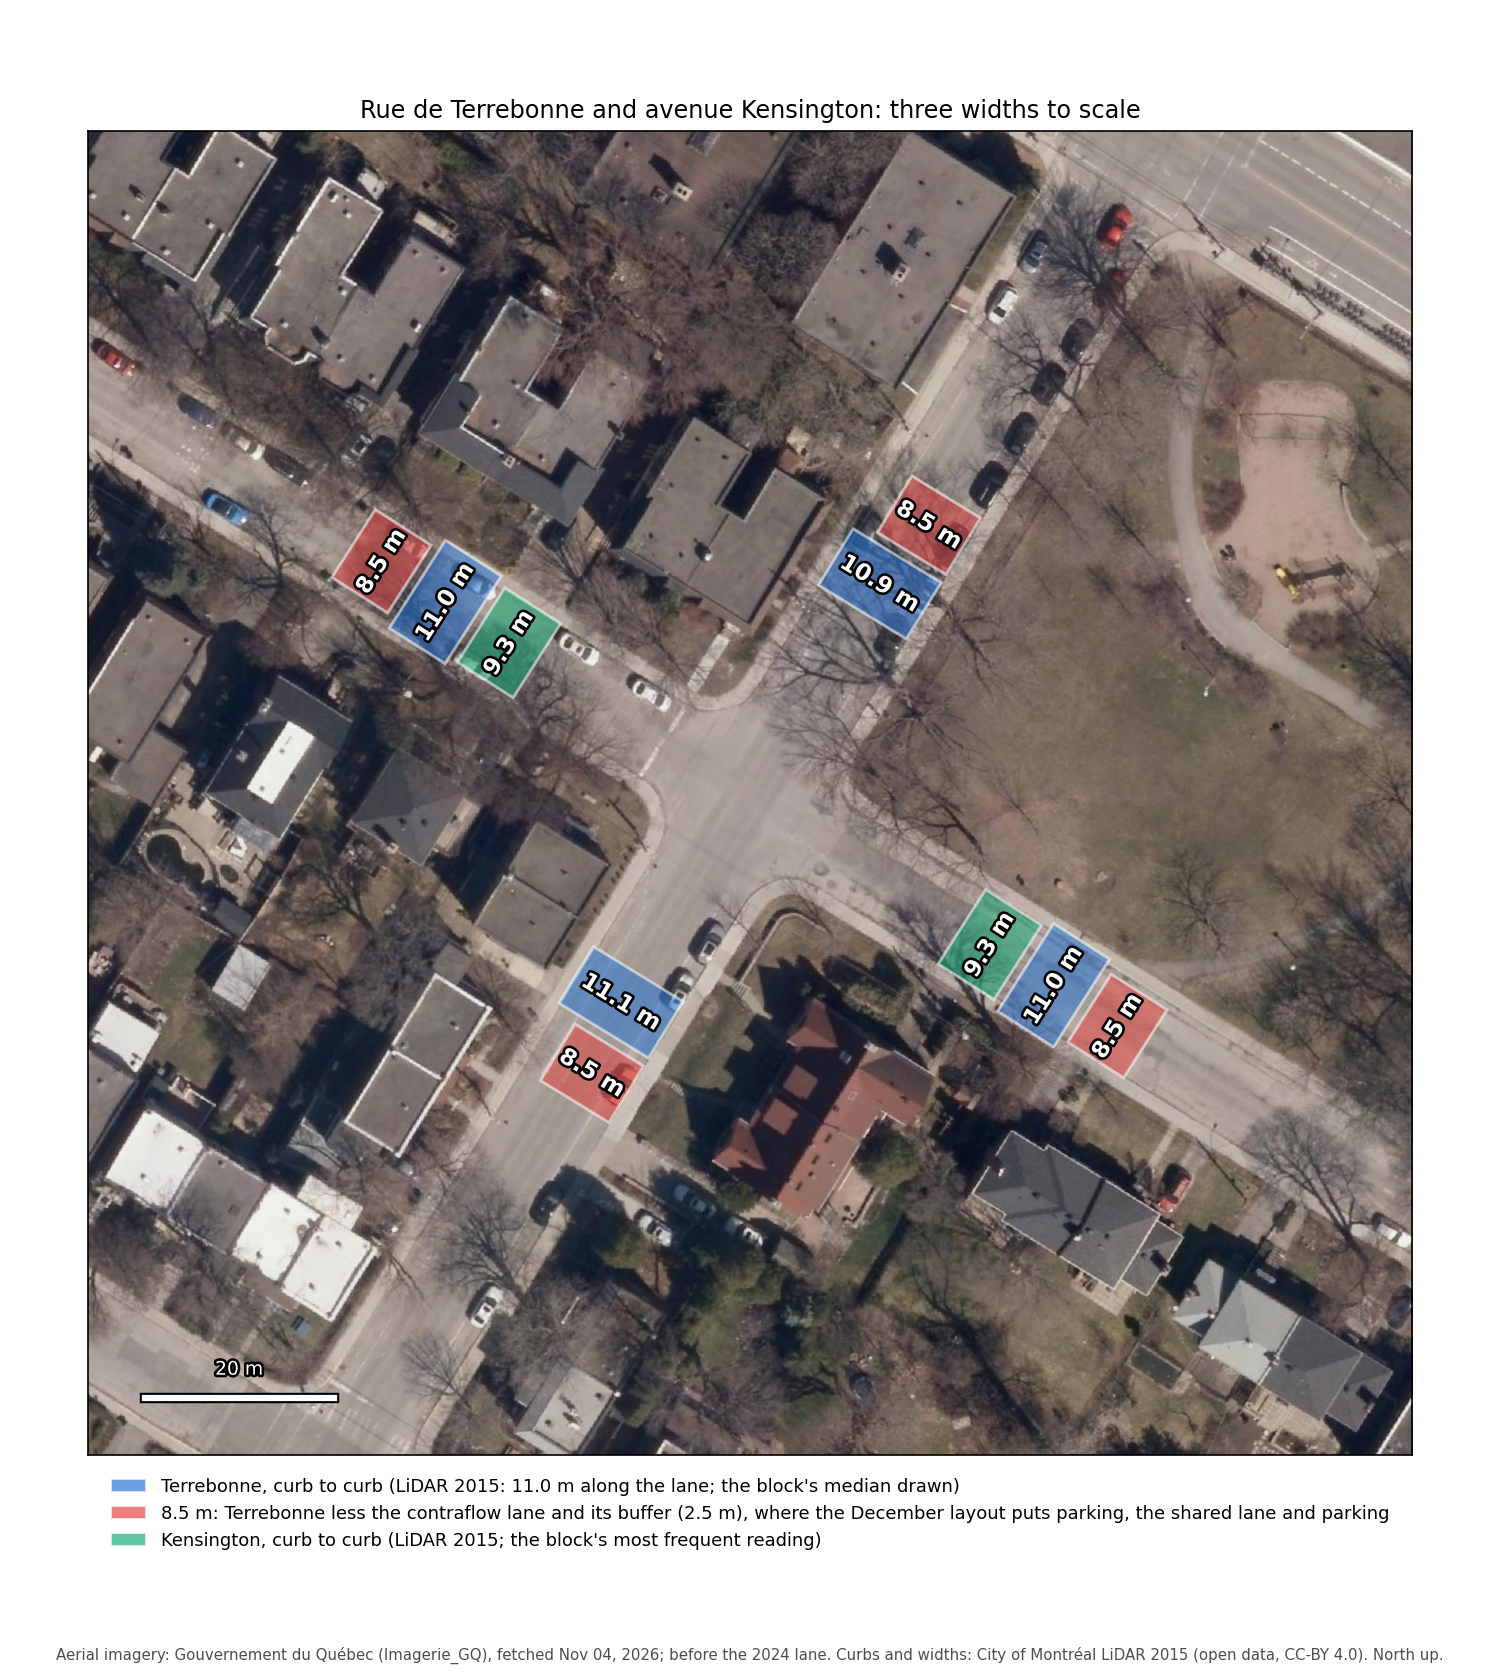
\includegraphics[height=0.6\textheight]{figures/cross_street_boxes_en.png}\caption{Rue de Terrebonne and avenue Kensington, the three widths to scale (aerial imagery: Gouvernement du Québec, Imagerie\_GQ, before the 2024 lane; curbs and widths: City LiDAR 2015).}\label{fig:boxes}\end{figure}

\textbf{What the cross streets show.} In one sentence: Due to the width of the roads and the allocation of 2.5 metres to the bike lane and buffer zone, the shared lane along Terrebonne will be around a metre narrower than the lanes shared by drivers and cyclists on the smaller side streets intersecting with Terrebonne. The author, who cycles the side streets, finds them already tight for a car to pass, even in summer; Terrebonne\textquoteright{}s shared lane for winter will be narrower still. Riding on the side streets is accepted practice: they are short blocks, used by drivers and cyclists to reach an address and, by cyclists, to move between the longer streets that carry bike lanes, so a driver held behind a cyclist is held for a block; Terrebonne is 2.4 km, and a driver held there is held for the length of the street. The arithmetic agrees with the experience. In the best case for a passing driver, the cyclist against the parked cars and one metre of clearance, a shared lane of 4.2 to 4.6 m leaves 2.5 to 2.8 m for the car; with the cyclist 0.5 m from the doors, 2.0 to 2.3 m. The winter layout\textquoteright{}s 3.5 m leaves 1.75 m and 1.25 m. The lane the winter layout draws for Terrebonne is therefore tighter than the shared lane of 45 of the 46 local cross-street blocks measured, and it is meant for the length of the street, in winter, where the cross streets serve a block or two.

\textbf{Caveats, for this part.} The cross streets\textquoteright{} parking bands are not marked: cars park at the curb, and a parked car takes 2.0 to 2.2 m with its mirrors, so the 2.4 m band is the drawing\textquoteright{}s figure applied for comparison. Snow windrows narrow Terrebonne and its cross streets alike. Only the first block on each side is measured; a street may change further from Terrebonne. The sign counts are an indicator of the parking regime, not a reading of the regulations. 2015 surface, as above.

\section*{By block}
{\small\begin{longtable}{@{}lrrrrrr@{}}\toprule Block (west to east) & kept/stations & curb--curb median (m) & p10--p90 & right-of-way (m) & sidewalk N (m) & sidewalk S (m)\\ \midrule
west end -- Belmore & 19/30 & 11.0 & 10.7--11.32 & 20.09 & 4.44 & 4.67 \\
Belmore -- Belmore & 4/12 & 11.0 & 10.9--11.31 & 28.48 & 4.6 & 12.03 \\
Belmore -- Coronation & 13/26 & 10.8 & 10.62--11.66 & 20.09 & 4.5 & 4.82 \\
Coronation -- Mayfair & 23/39 & 11.0 & 10.72--12.6 & 20.09 & 4.51 & 4.57 \\
Mayfair -- Mariette & 34/45 & 11.0 & 10.7--11.27 & 20.09 & 4.46 & 4.69 \\
Mariette -- Rosedale & 34/45 & 10.8 & 10.53--11.24 & 20.09 & 4.59 & 4.7 \\
Rosedale -- King-Edward & 27/44 & 11.0 & 10.76--11.78 & 20.09 & 4.46 & 4.63 \\
King-Edward -- Montclair & 34/46 & 11.1 & 10.73--12.55 & 20.09 & 4.39 & 4.61 \\
Montclair -- Walkley & 26/45 & 11.0 & 10.7--11.25 & 20.09 & 4.46 & 4.72 \\
Walkley -- Prince-of-Wales & 22/41 & 11.1 & 10.9--12.78 & 21.94 & 5.54 & 4.88 \\
Prince-of-Wales -- Cumberland & 17/36 & 11.0 & 10.8--11.3 & 20.09 & 4.67 & 4.6 \\
Cumberland -- Cavendish & 18/37 & 10.85 & 10.67--11.59 & 20.09 & 4.53 & 4.7 \\
Cavendish -- Bessborough & 19/37 & 11.0 & 10.6--11.52 & 20.09 & 3.75 & 5.49 \\
Bessborough -- Benny & 41/51 & 10.8 & 10.7--11.1 & 20.09 & 3.69 & 5.6 \\
Benny -- Madison & 68/79 & 11.0 & 10.7--11.43 & 20.09 & 3.56 & 5.47 \\
Madison -- Kensington & 26/42 & 11.1 & 10.7--12.65 & 20.09 & 4.39 & 4.7 \\
Kensington -- Grand & 25/42 & 10.9 & 10.7--12.8 & 20.09 & 4.38 & 4.75 \\
Grand -- Beaconsfield & 22/44 & 11.0 & 10.71--12.8 & 20.09 & 4.98 & 4.53 \\
Beaconsfield -- Hingston & 26/40 & 11.0 & 10.75--12.8 & 20.09 & 4.48 & 4.67 \\
Hingston -- Hampton & 28/49 & 11.15 & 10.87--12.73 & 20.09 & 4.34 & 4.66 \\
Hampton -- Royal & 27/49 & 11.0 & 10.8--12.52 & 20.1 & 4.38 & 4.75 \\
Royal -- Draper & 35/47 & 10.8 & 10.68--11.36 & 20.1 & 4.48 & 4.71 \\
Draper -- Melrose & 25/44 & 11.0 & 10.64--11.94 & 20.09 & 4.38 & 4.8 \\
Melrose -- Wilson & 25/41 & 11.0 & 10.6--12.6 & 20.1 & 5.23 & 3.97 \\
Wilson -- Harvard & 22/38 & 10.9 & 10.61--12.06 & 20.1 & 4.4 & 4.79 \\
Harvard -- d\textquoteright{}Oxford & 23/40 & 10.9 & 10.8--12.78 & 20.1 & 4.27 & 4.94 \\
d\textquoteright{}Oxford -- Marcil & 30/39 & 11.0 & 10.7--11.61 & 20.1 & 4.31 & 4.81 \\
Marcil -- Old Orchard & 24/39 & 11.0 & 10.56--11.37 & 20.1 & 4.4 & 4.69 \\
Old Orchard -- Girouard & 22/40 & 11.35 & 10.8--12.6 & 20.1 & 4.57 & 4.42 \\
\bottomrule\end{longtable}}

\section*{Caveats}
\begin{itemize}
\item The curb is read from a 0.25 m elevation grid: a single reading is good to about 0.2 m; the block medians are the figures to use.
\item 2015 surface, 2024 layout: the curbs have not moved; the lane markings of 2024 are not in the LiDAR.
\item Stations hidden by parked cars or trees are left out, not interpolated; blocks with few kept stations (Hingston--Hampton, Hampton--Royal) carry more uncertainty.
\item The right-of-way is the City\textquoteright{}s parcel geometry, not a survey.
\end{itemize}
\end{document}
